
\includegraphics[height=1.25cm]{images/pictograms/replication}
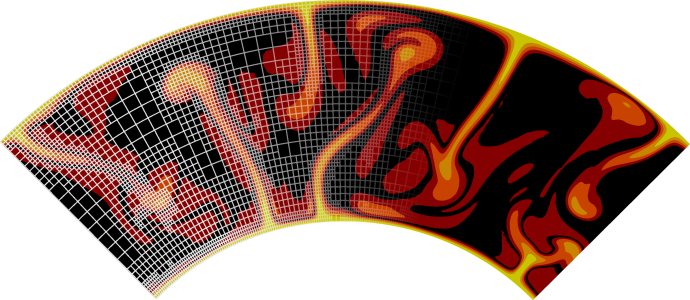
\includegraphics[height=1.25cm]{images/pictograms/aspect_logo}

\includegraphics[height=1.25cm]{images/pictograms/benchmark}

\includegraphics[height=1.25cm]{images/pictograms/under_construction}

\includegraphics[height=1.25cm]{images/pictograms/FEM}
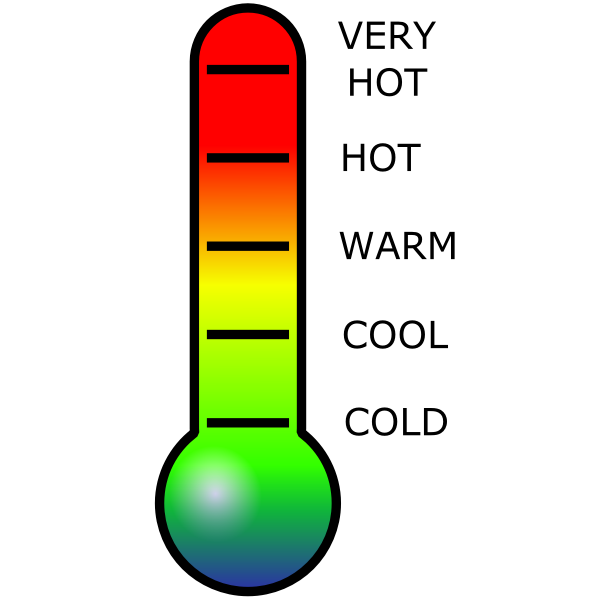
\includegraphics[height=1.25cm]{images/pictograms/temperature}

\includegraphics[height=1.25cm]{images/pictograms/paraview}

%%%%%%%%%%%%%%%%%%%%%%%%%%%%%%%%%%%%%%%%%%%%%%%%%%%%%%%%%%%%%%%%%%%%%%%%%%%%%%%%%%%%%%%%%%%%%%%%%%%

\begin{flushright} {\tiny {\color{gray} python\_codes/fieldstone\_149/text.tex}} \end{flushright}

\lstinputlisting[language=bash,basicstyle=\small]{python_codes/fieldstone_149/keywords.key}

\par\noindent\rule{\textwidth}{0.4pt}

\begin{center}
\inpython
{\small Code: \url{https://github.com/cedrict/fieldstone/tree/master/python_codes/fieldstone_149}}
\end{center}

\par\noindent\rule{\textwidth}{0.4pt}

{\sl This stone was developed in with input from Daniel Douglas}. 

\par\noindent\rule{\textwidth}{0.4pt}

%%%%%%%%%%%%%%%%%%%%%%%%%%%%%%%%%%%%%%%%%%%%%%%%%%%%%%%%%%%%%%%%%%%%%%%%%%%%%%%%%%%%%%%%%%%%%%%%%%%

In the {\pythonfile tools.py} there are two functions:
\begin{itemize}
\item \verb'merge_two_blocks': it takes as arguments two meshes and returns a single mesh in which 
the overlapping nodes of both have been merged and the global numbering and connectivity array computed.
\item \verb'export_to_vtu': it takes a mesh and exports it to vtu format.
\end{itemize}

%-------------------------------------------------
\section*{Joining two simple and identical meshes}

We start with two square meshes of resolution $20 \times 20$. This is implemented 
in {\pythonfile stone\_demo.py}. Note that the nodes of a block that are on the boundary 
('the hull') are flagged: indeed, only these are likely to be overlapping with a neighbouring 
block and merged.

\begin{center}
a)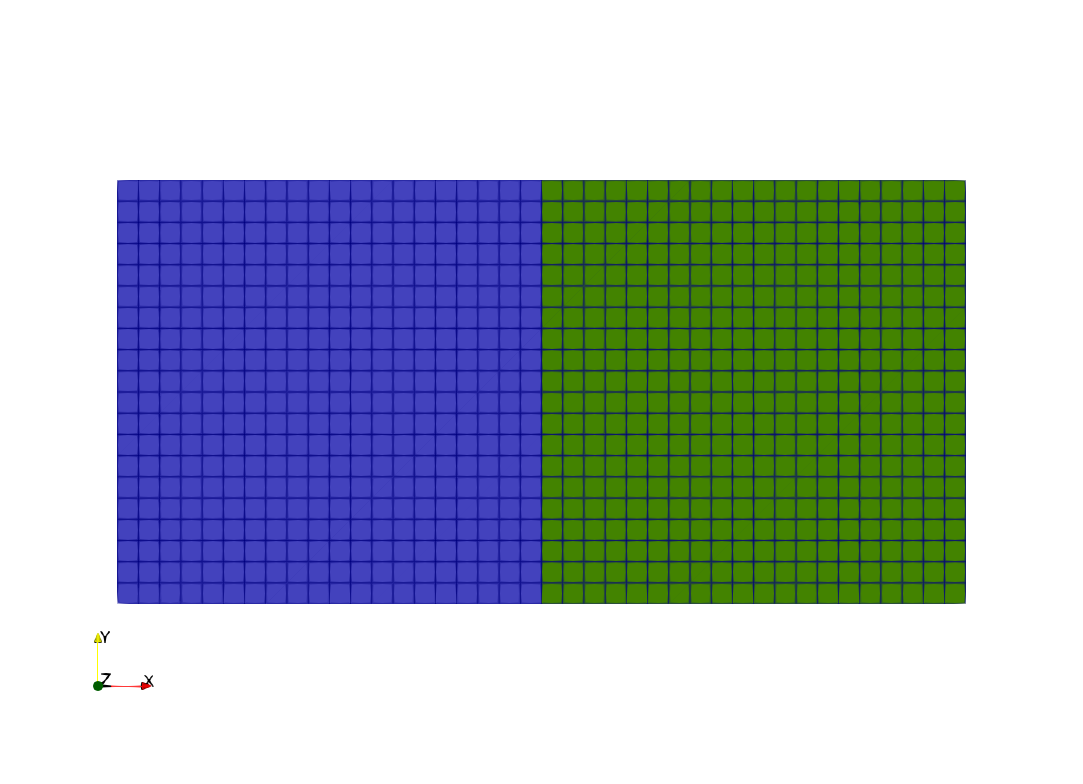
\includegraphics[width=8cm]{python_codes/fieldstone_149/results/meshing/one}
b)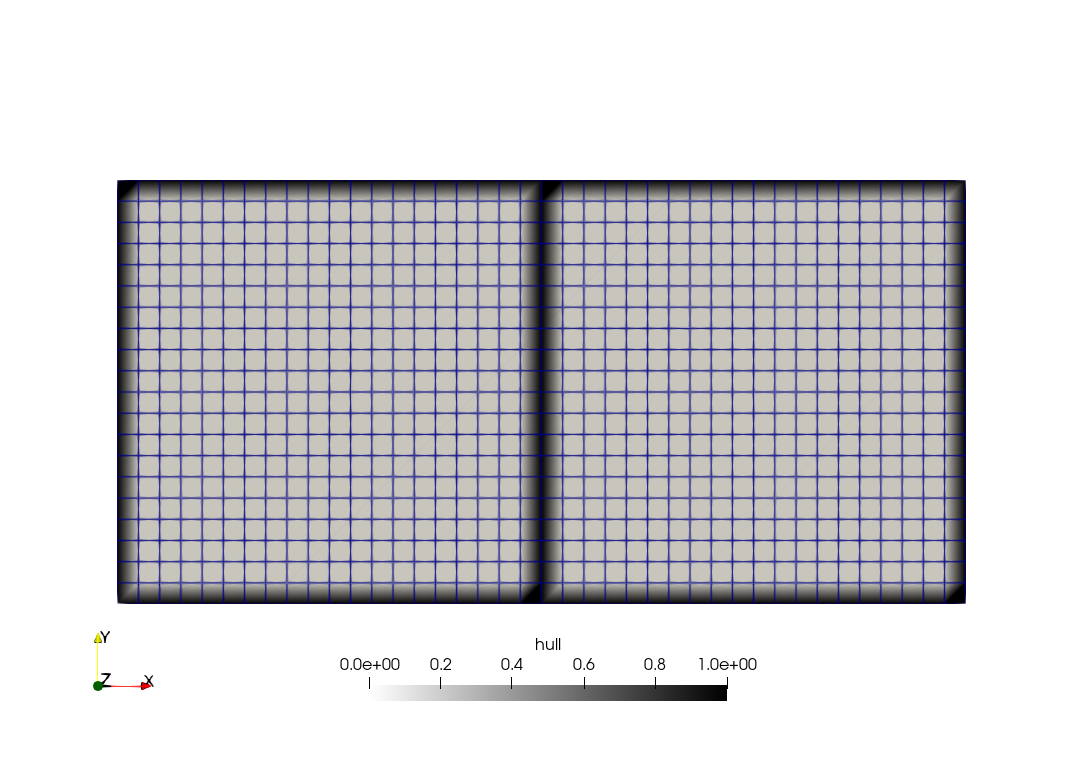
\includegraphics[width=8cm]{python_codes/fieldstone_149/results/meshing/two}\\
{\captionfont a) two individual meshes. b) final assembled mesh showing the hull flag. Note that the current algorithm does 
not unflag nodes that are no more on the boundary, it simply merges the two hull fields.}
\end{center}


%-------------------------------------
\section*{Joining multiple meshes}

This proto-mesh contains 8 elements and 14 points.

\begin{verbatim}
12---------------13
| \               |
|  10------------11 icon[0:m,0]=[0,1,6,5]
|   | \           | icon[0:m,1]=[1,2,7,6]
|   |  \          | icon[0:m,2]=[2,3,8,7]
|   |   \         | icon[0:m,3]=[3,4,9,8]
|   |    \        | icon[0:m,4]=[5,6,10,12]
5---6     8-------9 icon[0:m,5]=[6,7,8,10]    
|   | \   / \     | icon[0:m,6]=[8,9,11,10]
|   |   7-   \    | icon[0:m,7]=[10,11,13,12]
|   |     \   \   | 
0---1-----2----3--4
\end{verbatim}

\begin{center}
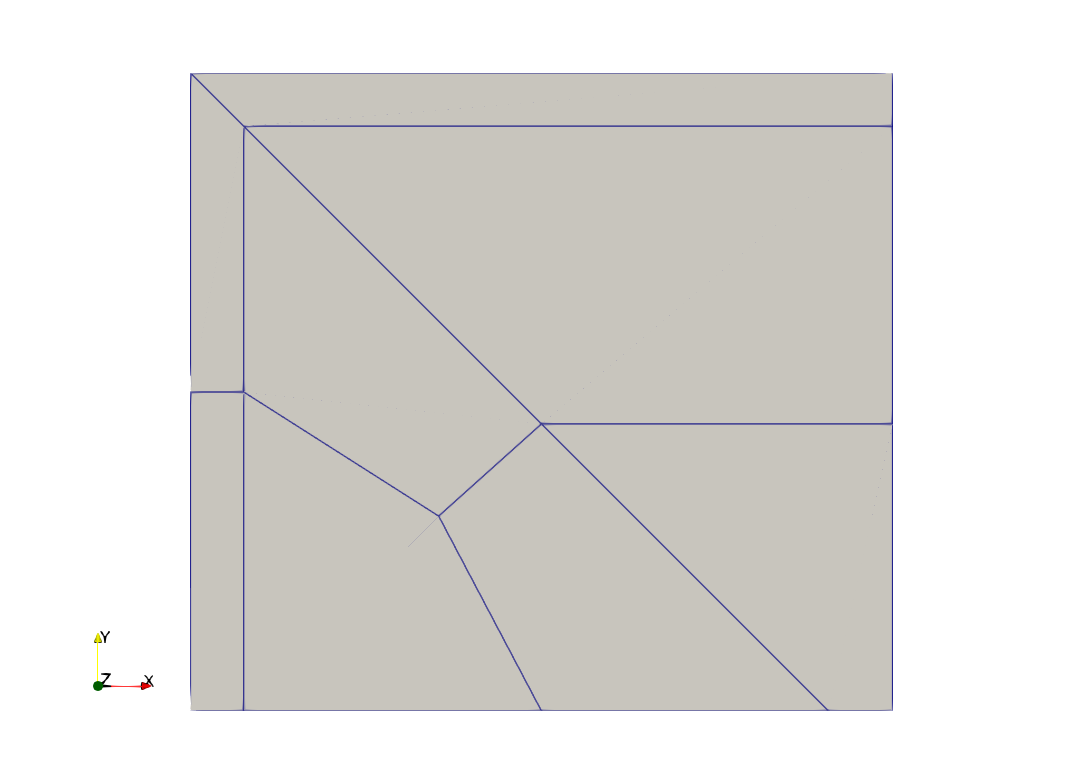
\includegraphics[width=8cm]{python_codes/fieldstone_149/results/meshing/mesh}
\end{center}

We then proceed by creating 8 blocks of resolution $10\times 10$. 
We then map them and finally assemble them one by one to obtain:

\begin{center}
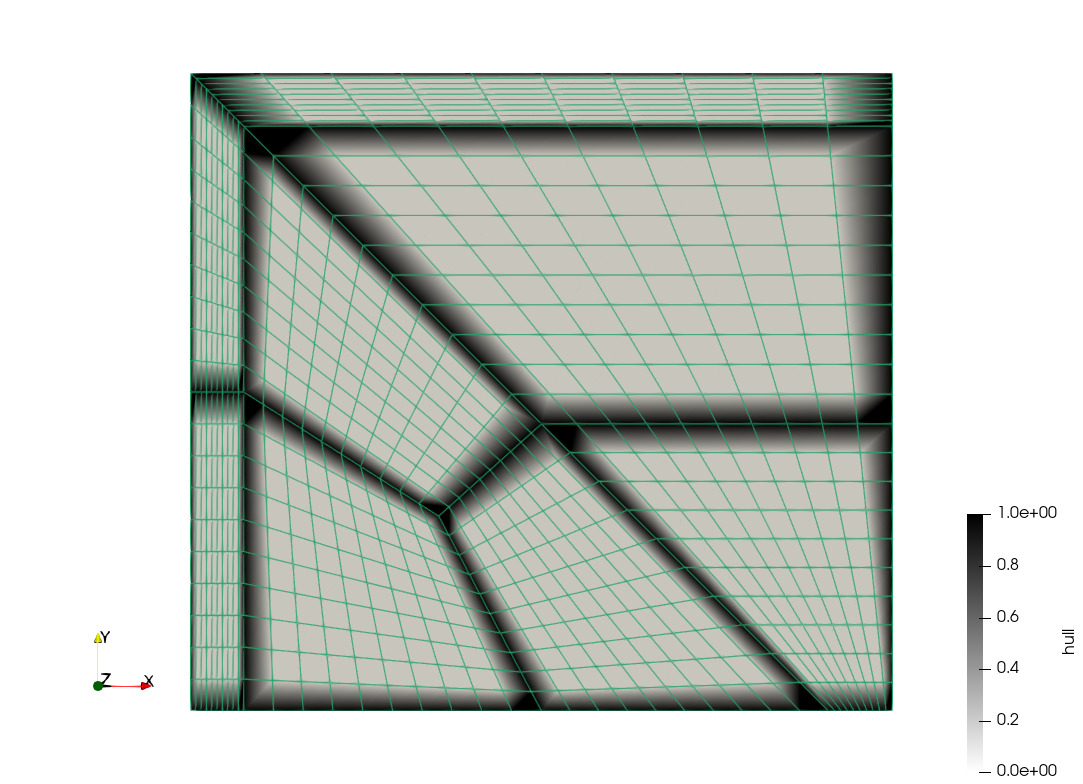
\includegraphics[width=8cm]{python_codes/fieldstone_149/results/meshing/vkkmesh}
\end{center}

%%%%%%%%%%%%%%%%%%%%%%%%%%%%%%%%%%%%%%%%%%%%%%%%%%%%%%%%%%%%%%%%%%%%%%%%%%%%%%%%%%%%%%%%%%%%%%%%%%%
\section*{About the code}

This is a rather peculiar approach that we take here. We wish to solve the 
temperature equation on the full domain $L_x \times L_y$ while 
we only wish to solve the Stokes equations on the domain composed of 
blocks 3 and 6. 

\begin{center}
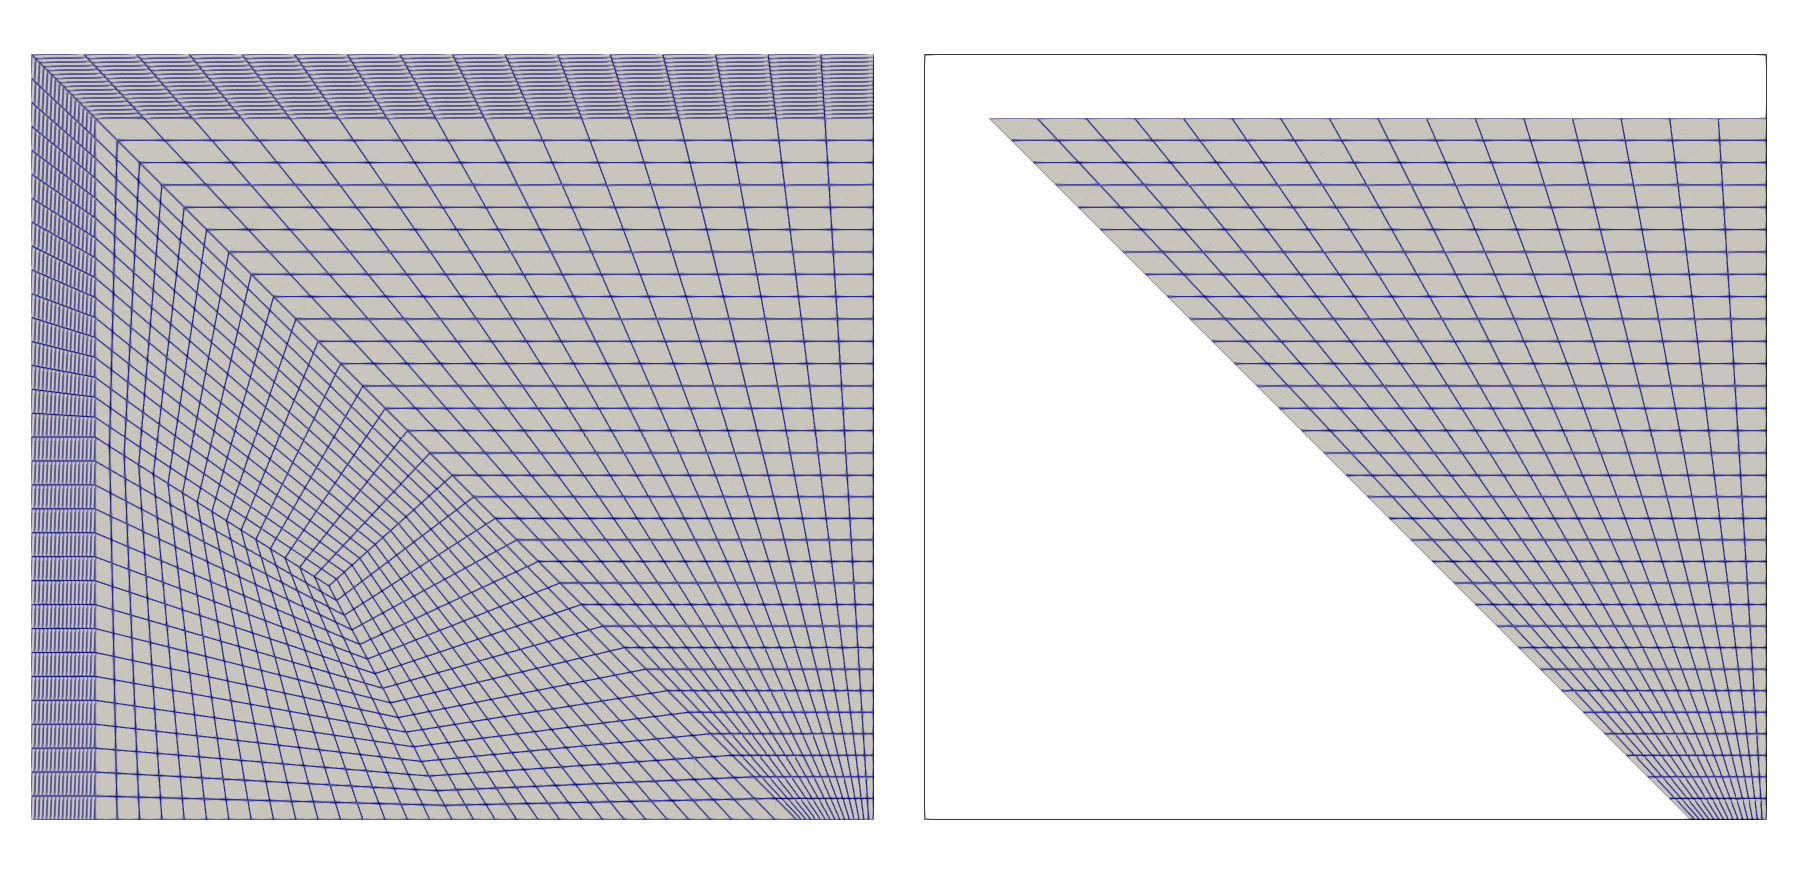
\includegraphics[width=14cm]{python_codes/fieldstone_149/results/meshing/meshes}
\end{center}


For simplicity (and because I have not yet implemented a version of the 
merging algorithm for second order elements), I will use 
the $Q_1^+\times Q_1$ pair for Stokes and $Q_1$ elements for the temperature.

Also, the steady state energy equation is solved. Since the (linear) Stokes equations 
do not depend on temperature, we then only need to solve the Stokes equations 
first and the energy equation second.

After the Stokes equations are solved we must transfer the velocity solution 
onto the temperature mesh. I have then created the {\tt mapping} array
that links each Stokes mesh point with a temperature mesh point.
Note that this algorithm is *very* slow and could certainly be improved
(currently about 500s for level=128!). 

Once the temperature equation is solved I also compute the nodal heat flux vector
$\vec{q}=-k \vec\nabla T$.

\newpage
%%%%%%%%%%%%%%%%%%%%%%%%%%%%%%%%%%%%%%%%%%%%%%%%%%%%%%%%%%%%%%%%%%%%%%%%%%%%%%%%%%%%%%%%%%%%%%%%%%%
\section*{Case 1a}

The Stokes equations are not solved. Instead the velocity field
is prescribed analytically everywhere in the domain, using the corner flow solution 
in the mantle wedge. 

The code uses analytical velocity from corner flow theory (see \stone~\ref{f68})
so the Stokes equations are (for now) not solved. 

%\begin{center}
%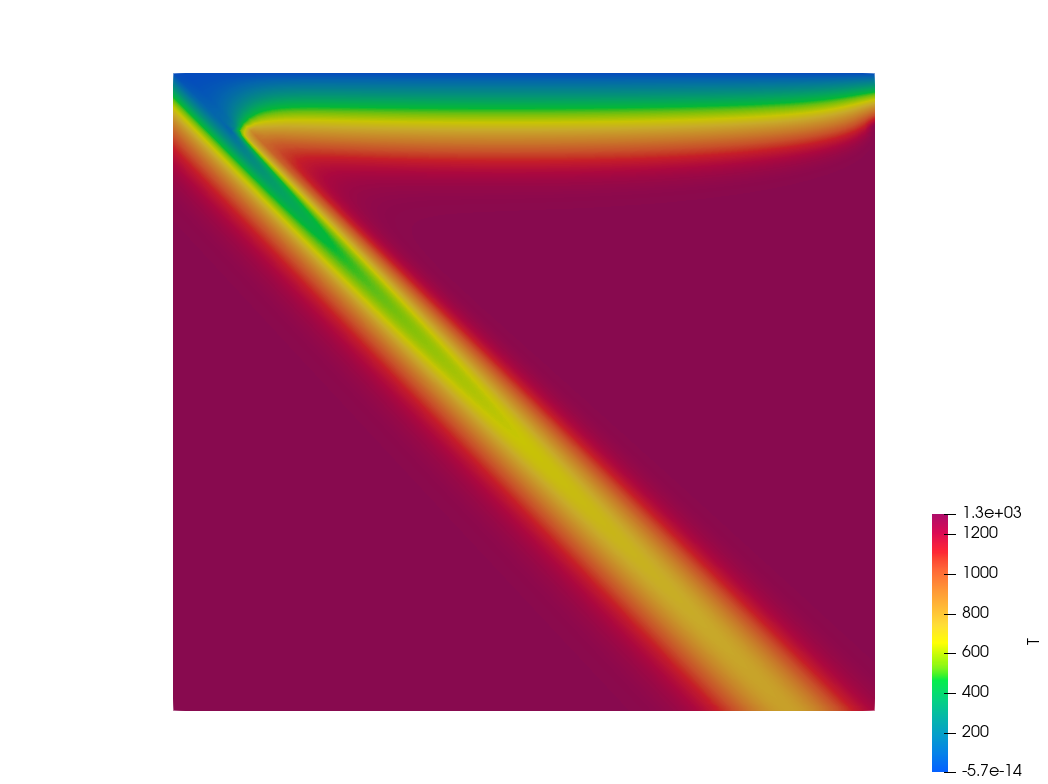
\includegraphics[width=8.5cm]{python_codes/fieldstone_149/results/case1a/temp}
%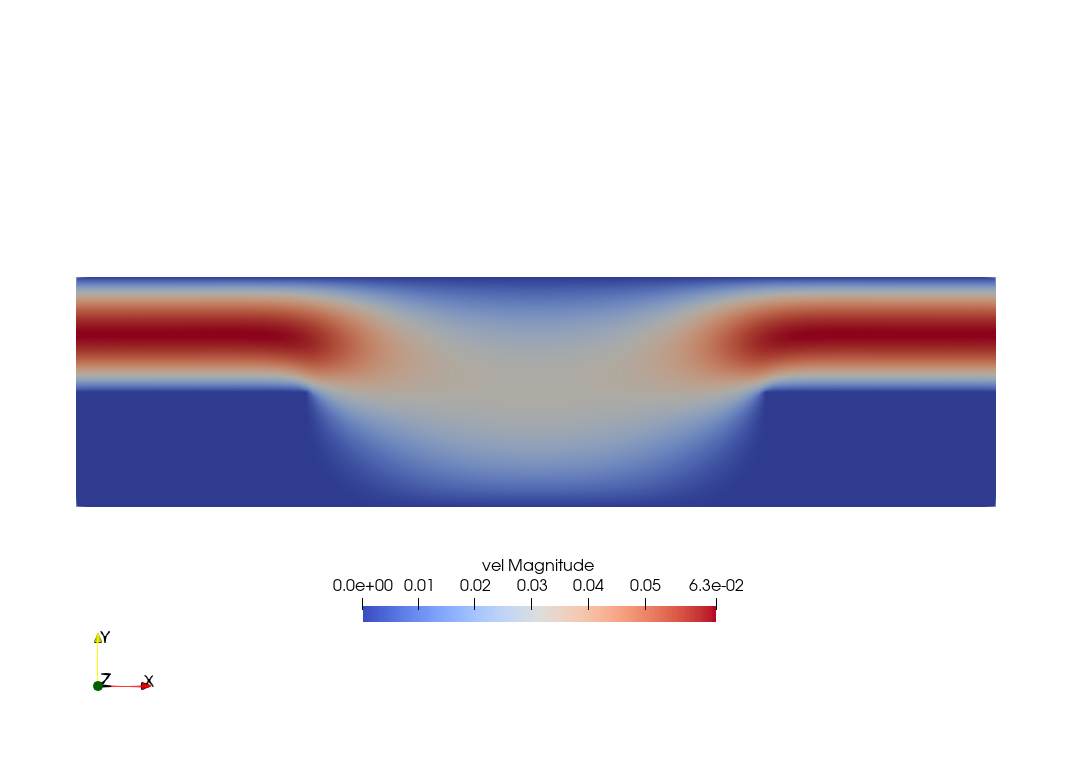
\includegraphics[width=8.5cm]{python_codes/fieldstone_149/results/case1a/vel}
%\end{center}

\begin{center}
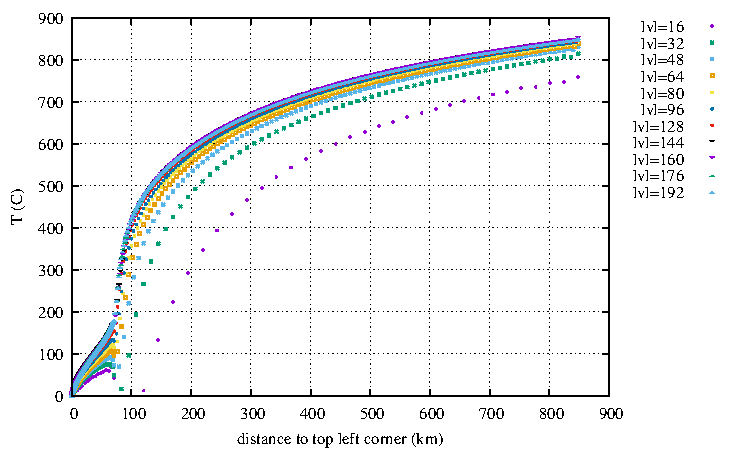
\includegraphics[width=8cm]{python_codes/fieldstone_149/results/case1a/diagT.pdf}
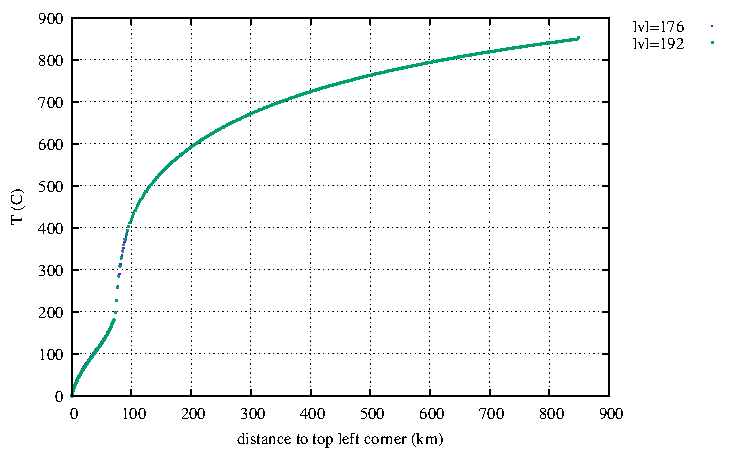
\includegraphics[width=8cm]{python_codes/fieldstone_149/results/case1a/diagT2.pdf}\\
{\captionfont We see that results seem to become resolution independent
when level$>160$.} 
\end{center}

%%%%%%%%%%%%%%%%%%%%%%%%%%%%%%%%%%%%%%%%%%%%%%%%%%%%%%%%%%%%%%%%%%%%%%%%%%%%%%%%%%%%%%%%%%%%%%%%%%%
\section*{Case 1b - dynamical flow in isoviscous wedge I}

This case is the same as 1a, except that the solution
for the wedge flow is determined by solving the Stokes equations while the Batchelor solution is
imposed on the inflow and outflow boundaries. This case tests the ability of the numerical method
to accurately reproduce the corner flow solution.

\newpage
%%%%%%%%%%%%%%%%%%%%%%%%%%%%%%%%%%%%%%%%%%%%%%%%%%%%%%%%%%%%%%%%%%%%%%%%%%%%%%%%%%%%%%%%%%%%%%%%%%%
\section*{Case 1c - dynamical flow in isoviscous wedge II} 

Same as case 1b, but with stress-free boundary conditions on the mantle wedge.

\begin{center}
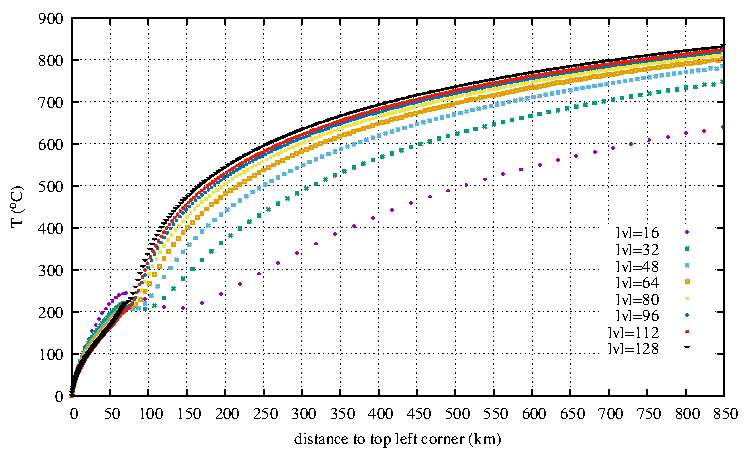
\includegraphics[width=8cm]{python_codes/fieldstone_149/results/case1c/diagT.pdf}
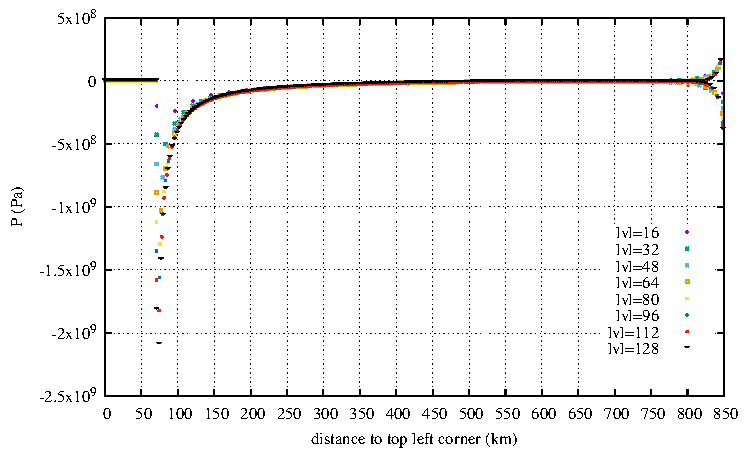
\includegraphics[width=8cm]{python_codes/fieldstone_149/results/case1c/diagP.pdf}\\
{\captionfont Measurements on the diagonal.} 
\end{center}

\begin{center}
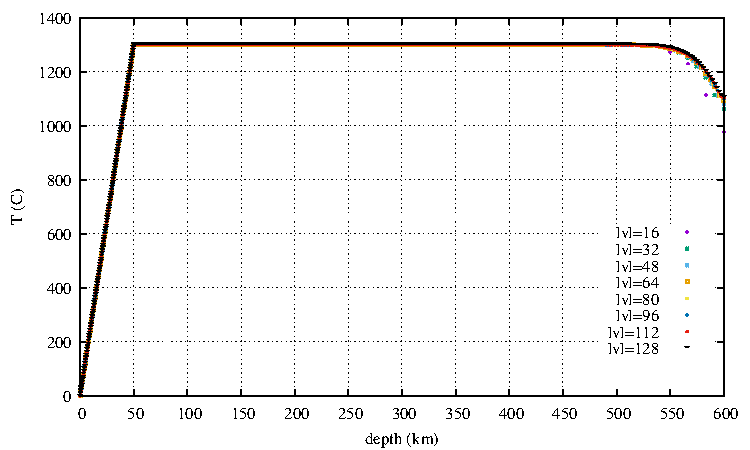
\includegraphics[width=8cm]{python_codes/fieldstone_149/results/case1c/rightT.pdf}
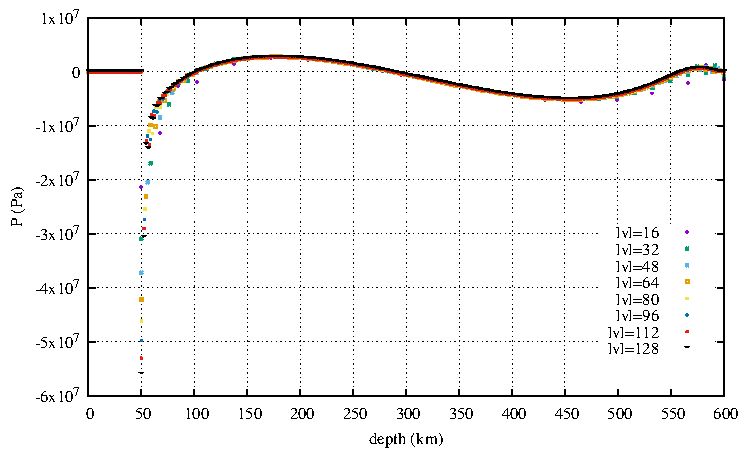
\includegraphics[width=8cm]{python_codes/fieldstone_149/results/case1c/rightP.pdf}\\
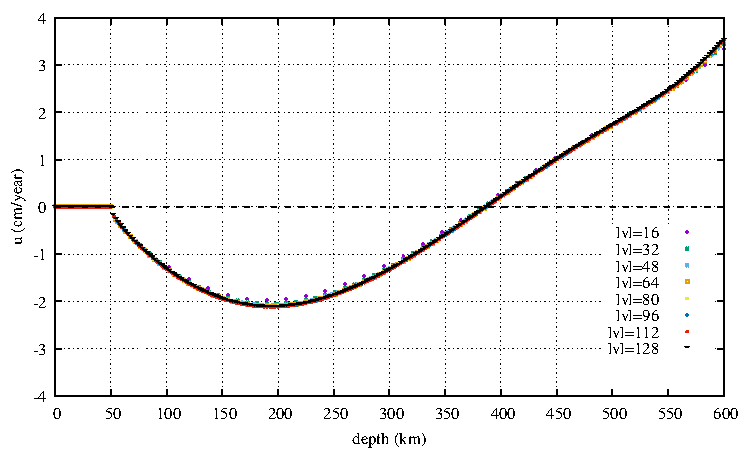
\includegraphics[width=8cm]{python_codes/fieldstone_149/results/case1c/rightu.pdf}
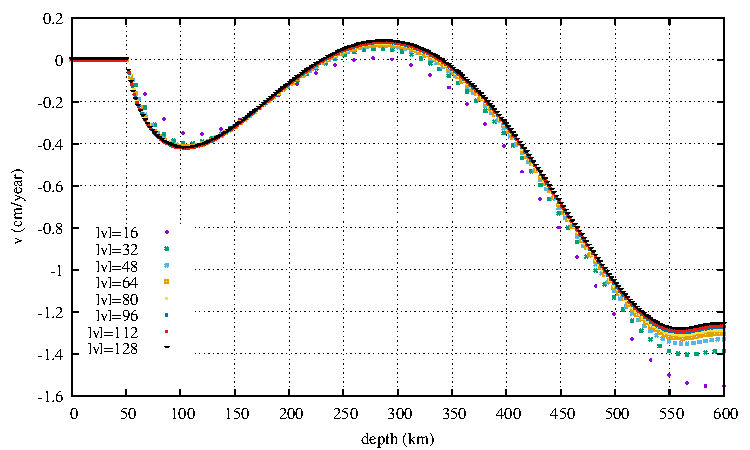
\includegraphics[width=8cm]{python_codes/fieldstone_149/results/case1c/rightv.pdf}\\
{\captionfont Measurements on the right side of the domain.}
\end{center}

There seems to be a pressure instability/mode towards the bottom?!
Is this because of the element?











\newpage
%%%%%%%%%%%%%%%%%%%%%%%%%%%%%%%%%%%%%%%%%%%%%%%%%%%%%%%%%%%%%%%%%%%%%%%%%%%%%%%%%%%%%%%%%%%%%%%%%%%
\par\noindent\rule{\textwidth}{0.4pt}

\vspace{.5cm}

\begin{center}
\fbox{\begin{minipage}{0.9\textwidth}
{\color{teal}To Do, open questions, future work?}
\begin{itemize}
\item use f131 P1 to P2 tool to make Q1 to Q2 ?
\item redo figures with appropriate colors
\item redo (some) benchmark measurements?
\item improve mapping algo?
\item is it worth moving to Q2Q1 ? what about the weird pressure error of Q1+xQ1 ? 
\end{itemize}
\end{minipage}}
\end{center}

%%%%%%%%%%%%%%%%%%%%%%%%%%%%%%%%%%%%%%%%%%%%%%%%%%%%%%%%%%%%%%%%%%%%%%%%%%%%%%%%%%%%%%%%%%%%%%%%%%%
\vspace{.5cm}

\Literature:\\
\fullcite{vack08}\\
\fullcite{vatc23}

